\chapter{Conclusion}
\label{c:DandC}

In this thesis, searches for the production of four top quarks at $\sqrt{s}=8$~TeV and $\sqrt{s}=13$~TeV at the CMS experiment at CERN were presented. In addition to this, a phenomenological interpretation of the results at $\sqrt{s}=8$~TeV in the context of a simplified model with sgluon particles was presented.

In Chapter~\ref{c:theory}, the theory background of the SM was discussed. There was a more focussed look at top physics, alongside a discussion of the models of physics beyond the SM which have four top signatures such as top quark compositeness and the pair production of top-philic sgluons. 
In Chapter~\ref{c:det}, the LHC and the associated accelerator complex were described. More specifically the CMS detector was described in terms of each of its sub-detectors, from tracking to electromagnetic and hadronic calorimetry and muon detection.
In Chapter~\ref{c:recon}, the reconstruction of physics objects from the CMS detector readout, such as electrons, muons and jets, was described.
The analysis strategy and techniques used when searching for \tttt production in this thesis were described in Chapter~\ref{c:ana}. This included discussion of the background processes which can mimic \tttt production in the detector, corrections to the simulation, multivariate techniques and the statistical tools used.
The analysis and results from \runone at $\sqrt{s}=8$~TeV, the search for the production of \tttt in the single lepton channel, were presented in Chapter~\ref{c:Run1}. This result was used alongside a CMS same-sign dilepton analysis to place constraints on the mass of the sgluon and its coupling to the top quark.
Finally, the results from the search for the production of four top quarks at $\sqrt{s}=13$~TeV in \runtwo were presented in Chapter~\ref{c:Run2}. Many cross checks were performed on the analysis and it was shown to be stable and the observed data were well modelled by simulation. Also, a combination of this search with an opposite-sign and a same-sign dilepton analysis, was presented, which produces the world's current tightest limit on the production rate of four top quarks.

\section{Summary of results}

In \runone and \runtwo, the main background after the baseline selection requirement was \ttbar production where the extra jets required to meet the selection requirements tend to come from ISR and FSR. Smaller contributions to the background came from single top production, W and Z boson production, and even less so from \ttH, \ttW, \ttZ. 

One BDT was used to identify hadronically decaying top quarks and a second BDT was used to separate signal and background using variables which described the event activity, b-jet content and variables derived from the hadronic top BDT.

At $\sqrt{s}=8$~TeV, the BDT templates were split into \njets categories only and a simultaneous fit was made in the electron and muon channels. This resulted in a $95\%$ CL on $\sigmatttt~/~\sigmattttSM$ of 25 ($24.6\pm13$) observed (expected) which corresponds to a cross section of 32~\fb ($32.0\pm17$~\fb) observed (expected). This result was both competitive and consistent with the other limits on \tttt production in \runone from both CMS and ATLAS.

At $\sqrt{s}=13$~TeV, the analysis saw improvements from using larger samples of simulated data and better modelling of \tttt by using a NLO sample rather than LO. Improvements were also made to the modelling of b-tagging by using scale factors which correct the CSV discriminator distributions.
The variables input into the event-level BDT were reoptimised and the BDT was shown to be very stable to variations in its hyperparameters. Further to the categorisation of the BDT templates in \njets categories in the \runone analysis, the templates were also categorised by \nMtags categories which was motivated by the increase in sensitivity seen by other searches for \tttt production. A simultaneous fit was performed in the electron and muon channels in all \njets and \nMtags categories which resulted in a $95\%$ CL limit of $16.8~(16.0^{+9.8}_{-5.5})\times \sigmattttSM$ observed (expected) in the single lepton channel. This result was further combined with an OS-dilepton and a SS-dilepton search for four top quark production in CMS, which resulted in an expected limit of $7.2~(7.5^{+4.1}_{-2.5})\times \sigmattttSM$ observed (expected) which equates to a cross section of 66~fb (69$^{+37}_{-23}$~fb) observed (expected) - the world's tightest limit on \tttt production at present.


\begin{figure}[ht!]
\begin{center}
    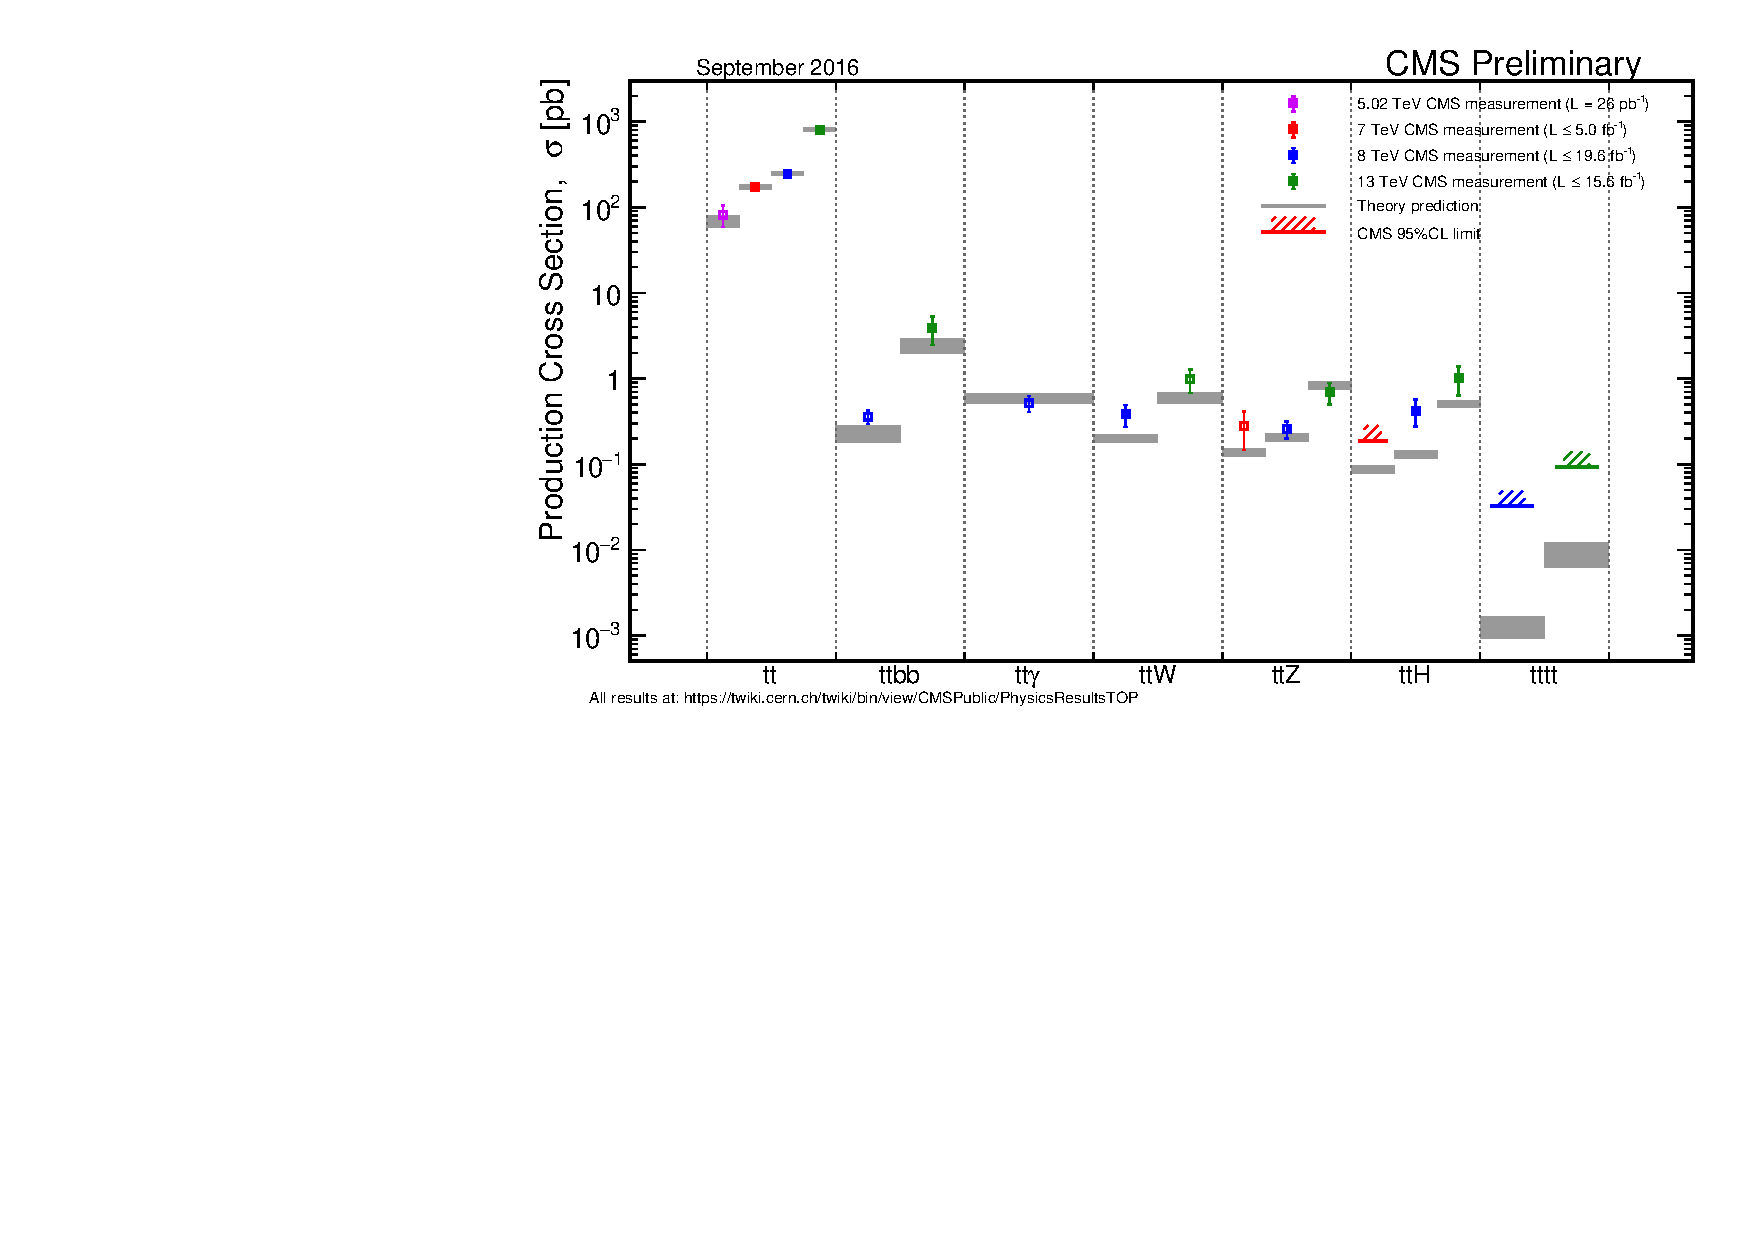
\includegraphics[width=0.97\textwidth]{images/Conclusion/ttplusx_staircase.pdf}
    \caption{Top quark production cross section summary plot showing measurement using square points and $95\%$ upper limits by a hatched band. Theory predictions are shown where the grey band represents the uncertainty on the prediction~\cite{topSumTwiki}.}
    \label{fig:ttbarXstairway}
\end{center}
\end{figure}

Figure~\ref{fig:ttbarXstairway} shows the CMS top quark cross section measurements as of September 2016. This figure highlights how much larger the main background of \ttbar production is compared to \tttt production.
Evidence has been seen for some of the rarer top physics processes, \ttbb, \ttgam, \ttW, \ttZ and \ttH, shown in Fig.~\ref{fig:ttbarXstairway}. It can be seen that the production of \tttt is at least an order of magnitude smaller that the other rare top physics processes being studied. The limit at $\sqrt{s}=8$~TeV is from the analysis in this thesis and the limit shown for $\sqrt{s}=13$~TeV on the figure comes from the preliminary result~\cite{CMS-PAS-TOP-16-016} which was released before changing the b-tagging scale factors for the final result which is presented in Chapter~\ref{c:Run2}.

\section{Future prospects}

Figure~\ref{fig:ttbarXstairway} shows the expected $95\%$ upper limit on $\sigmatttt~/~\sigmattttSM$ against integrated luminosity, where the luminosity has been artificially enhanced within the Higgs Combine Tool. The dashed black line indicates the \runtwo result from Chapter~\ref{c:Run2}. It can be seen that, in the absence of a signal, without any further enhancements or optimisations to the analysis workflow, the expected limit should decrease down the level of the SM expectation simply by increasing the amount of data up to 30-100~\fbinv.

\begin{figure}[ht!]
\begin{center}
    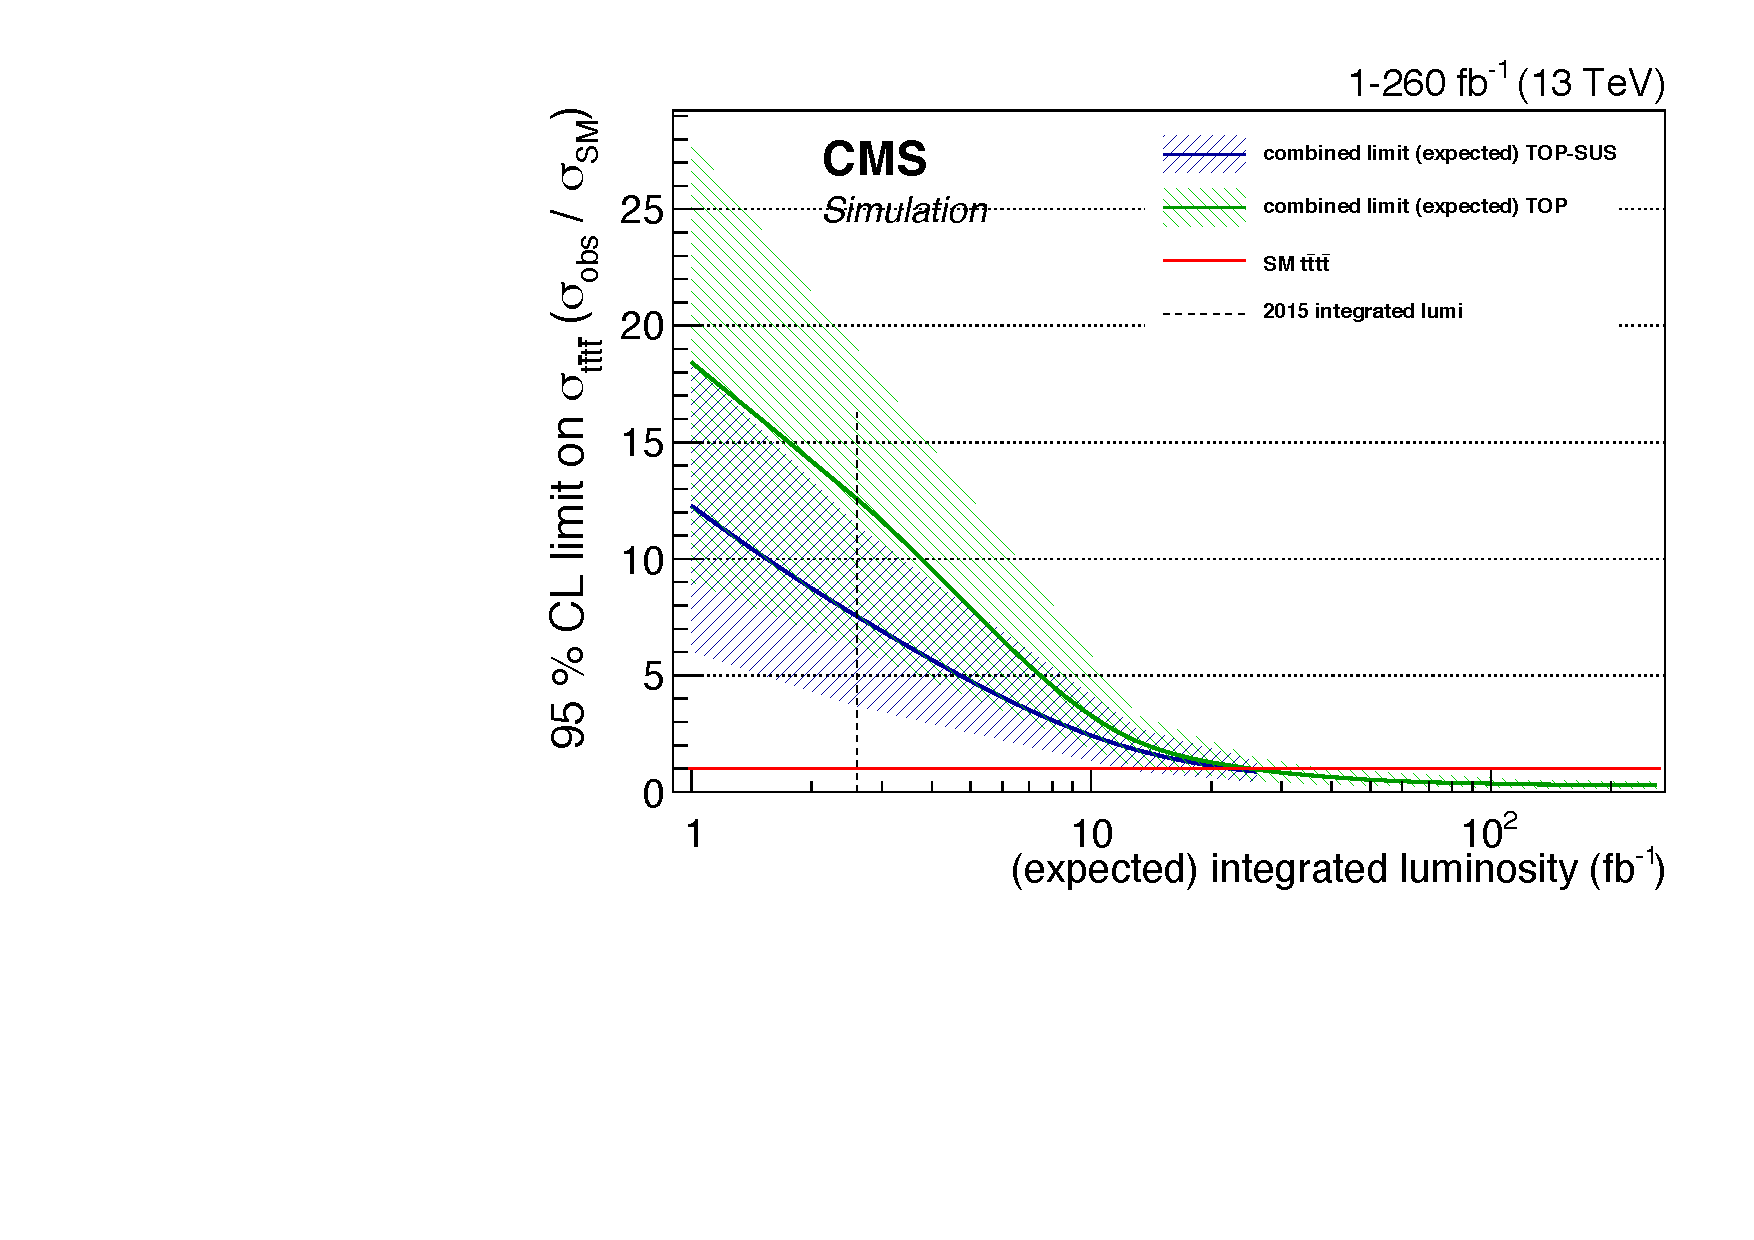
\includegraphics[width=0.97\textwidth]{images/Conclusion/combined_limitvslumi.pdf}
    \caption{Extrapolated limits on four-top-quark production using the single lepton and opposite-sign dilepton analyses (denoted TOP and in green) and using the single lepton, opposite-sign dilepton and the same-sign dilepton analyses (denoted SUS and in blue). The red line indicate the SM production rate. See Table~\ref{tab:CmsAtlasSum} for details of these analyses using 2.6~\fbinv.}
    \label{fig:ttbarXstairway}
\end{center}
\end{figure}

This suggests that it may be possible to produce a limit consistent with $1 \times \sigmattttSM$ using the dataset which has been collected by CMS in 2016 which has 41.1~\fbinv of data as shown in Figure~\ref{fig:Lumi}.\\

It may be possible to optimise the analysis further by including the $\njets=5$ category, as in Ref.~\cite{ATLAS-CONF-2016-020}, to further constrain \ttbar. Many four-top-quark searches have also categorised in \HT and \MET~\cite{ATLAS-CONF-2016-020,Chatrchyan:2013fea}. So far the hadronic top quark BDT has been trained on top quarks from \ttbar events, but it may be beneficial to also train on hadronic tops from \tttt events. It may be possible to find more discriminating variables for use in the event-level BDT, or to use a different multivariate algorithm such as a neural network which uses linear combinations of the inputs at each layer rather than the single requirement in each variable used by BDTs. Lastly, the systematic uncertainties used in Chapter~\ref{c:Run2} were potentially larger than necessary to sufficiently model the simulation. There were several shape systematic uncertainties which could potentially be substituted into normalisation uncertainties.\\

In summary, the analyses in this paper have produced the most stringent limit on four-top-quark production to date. This result constrains what BSM scenarios are possible, for instance by reducing the allowable phase-space of the sgluon particle, in mass and coupling to the top quark, as seen in Chapter~\ref{c:pheno}. It is possible that, with the enhancements to the analysis mentioned and the much larger dataset collected by CMS in 2016, direct evidence of the production of four top quarks is within our reach.



